\documentclass[11pt, twocolumn]{article}

\usepackage[spanish]{babel}
\usepackage[none]{hyphenat}
\usepackage[left=1.2cm, right=1.2cm, top = 2cm, bottom=2.5cm]{geometry}
% \usepackage{setspace}
\usepackage{parskip}
\usepackage[export]{adjustbox}
\usepackage{enumitem}
\usepackage{listings}
\usepackage[dvipsnames]{xcolor}
\usepackage{fancyhdr}
\usepackage{graphicx}
\usepackage{caption}
% \usepackage{subcaption}
% \usepackage{wrapfig}
% \usepackage{multirow, makecell}
% \usepackage{float}
% \usepackage{amsmath} 
% \usepackage{amsfonts}
\usepackage[hidelinks]{hyperref}
\usepackage{csquotes}

\newcommand{\linejump}{\hfill \break}
\renewcommand{\thefootnote}{\fnsymbol{footnote}}
% \newcommand{\unit}[1]{\ensuremath{\, \mathrm{#1}}}

\definecolor{dkgreen}{rgb}{0,0.6,0}
\definecolor{gray}{rgb}{0.5,0.5,0.5}
\definecolor{mauve}{rgb}{0.58,0,0.82}
\lstset{
  language=Java,
  aboveskip=3mm,
  belowskip=3mm,
  showstringspaces=false,
  columns=flexible,
  basicstyle={\tiny\ttfamily},
  numbers=none,
  numberstyle=\tiny\color{gray},
  keywordstyle=\color{blue},
  commentstyle=\color{dkgreen},
  stringstyle=\color{mauve},
  breaklines=true,
  breakatwhitespace=true,
  tabsize=2
}

\sloppy
\setlength{\parindent}{0cm}
\setlength{\columnsep}{0.5cm}
\decimalpoint
\graphicspath{{img/}}

\hypersetup{colorlinks=true, urlcolor=blue, citecolor=blue}
\urlstyle{same}

\pagestyle{fancyplain}
\fancyhf{}
\fancyhead[L]{\scriptsize 
  Universidad Nacional Autónoma de México \\
  Laboratorio de Programación Orientada a Objetos \\
  M.C. Leonardo Ledesma Dominguez
}
\fancyhead[R]{\thepage}

\begin{document}
  \twocolumn[
    \centering
    Acosta Porcayo Alan Omar, Gutiérrez Grimaldo Alejandro, Medina Villa Samuel

    \linejump

    \textbf{\LARGE{Práctica 11. Manejo de Archivos}} \\
    
    \linejump
  ]
      
  \footnotetext{
    \scriptsize 
    Acosta Porcayo Alan Omar Ing. en Computación 320206102 \\
    Gutiérrez Grimaldo Alejandro Ing. en Computación 320282098 \\
    Medina Villa Samuel Ing. en Computación 320249538
  }
        
  \fancyfoot{}

  \section*{Resumen}
  Esta práctica consistirá en implementar de manera eficiente el intercambio de datos entre un programa orientado a objetos y fuentes externas como archivos y la entrada/salida estándar. Las actividades planificadas incluirán la creación de archivos de texto plano, la lectura de datos desde estos archivos y la escritura de información en ellos.

  Durante este trabajo, se aplicarán principios solidos de programación orientada a objetos para estructurar y gestionar de manera efectiva la información antes de la lectura o escritura en los archivos. Se espera que esta experiencia fortalezca las habilidades en el manejo de archivos y la aplicación práctica de conceptos clave de programación orientada a objetos en el contexto específico del intercambio de datos con fuentes externas.
  
  \section*{Introducción}
  En el desarrollo de programas, la interacción con el entorno es esencial. La manipulación de archivos se convierte en un componente clave, utilizando flujos de datos para la transferencia de información entre el programa y fuentes externas. Este proceso implica el manejo de flujos de entrada, provenientes de la fuente, y flujos de salida, hacia el repositorio.

  \subsection*{Archivos}
  Los archivos, como objetos informáticos, almacenan datos y comandos. En este contexto, se abordan conceptos fundamentales como la unicidad del nombre de archivo y la identificación del tipo mediante extensiones. Este estudio se enfoca en JAVA, pero se deja a criterio del profesor el uso de otros lenguajes orientados a objetos.

  \subsection*{Flujos de Datos en Java}
  La gestión de entradas y salidas de datos en Java se realiza mediante streams. Se exploran cuatro jerarquías de clases: flujos de bytes para datos binarios y flujos de caracteres para datos textuales, cada uno con sus respectivas clases derivadas.

  \subsection*{Clase \textit{File} y Gestión de Archivos}
  La clase \textit{File} facilita la creación, borrado y otras funciones sobre archivos y carpetas. Su instancia no genera archivos, solo referencia objetos, y su utilidad radica en la manipulación explícita mediante métodos específicos.

  \subsection*{Manipulación de Flujos de Bytes y Caracteres}
  Se exploran clases como \textit{FileOutputStream} y \textit{FileInputStream} para escribir y leer flujos de bytes desde y hacia archivos de texto plano. Asimismo, clases como \textit{FileWriter}, \textit{BufferedWriter}, y \textit{PrintWriter} se emplean para manipular flujos de caracteres, permitiendo una escritura eficiente y sencilla en archivos.

  \subsection*{Clases \textit{Reader} y \textit{Scanner}}
  Las clases \textit{Reader}, como \textit{FileReader} e \textit{InputStreamReader}, se destacan en la lectura de flujos de caracteres, mientras que la clase \textit{Scanner} simplifica la lectura de flujos de bytes, proporcionando métodos como \textit{next()} y \textit{hasNext()}.
  
  \subsection*{Clase \textit{Console} y Serialización}
  La clase \textit{Console} facilita la lectura desde la línea de comandos, mientras que la serialización se presenta como un mecanismo esencial para preservar el estado de objetos mediante la conversión a secuencias de bytes, con consideraciones sobre la transitividad de referencias y el uso de la palabra clave \textit{``transient''} para objetos no serializables.

  \section*{Objetivos}
  \begin{itemize}
    \item Implementar la capacidad del programa para crear archivos de texto plano de manera eficiente y estructurada.
    \item Implementar clases como \textit{FileOutputStream} y \textit{FileInputStream} para la manipulación de flujos de bytes en archivos de texto plano.
    \item Implementar clases como \textit{FileReader}, \textit{InputStreamReader} y \textit{Scanner} para la lectura de flujos de caracteres y bytes.
    \item Implementar el intercambio de datos (lectura y escritura) entre fuentes externas (archivos y/o entrada y salida estándar) y un programa (en un lenguaje orientado a objetos)
  \end{itemize}

  \section*{Metodología}
  \textit{\textbf{Contact.java}}
  \begin{lstlisting}
import java.io.Serializable;

public class Contact implements Serializable {
  private String name, mobile, email;
  private transient String address;
   
  public Contact(String n, String t, String e) {
    this.name = n;
    this.mobile = t;
    this.email = e;
  }

  public Contact() {}

  public void setAddress(String s) {this.address = s;}
  public String getAddress() {return address;}

  //public void setName(String s) {this.name = s;}
  public String getName() {return name;}

  public String getMobile() {return mobile;}
  public String getEmail() {return email;}

  public String toString() {
    return "El contacto en la agenda POO: \nSe llama:" + this.name + 
        "\nSu telefono: " + this.mobile	+ 
        "\nSu correo: " + this.email + 
        "\nSu domicilio: "+ this.address;
  }
}
  \end{lstlisting}

  \textit{\textbf{Server.java}}
  \begin{lstlisting}
import java.io.ObjectOutputStream;

import java.net.ServerSocket;
import java.net.Socket;

import java.util.ArrayList;
import java.util.Scanner;

public class Server {
  public static void main(String[] args) throws Exception {
    ArrayList<Contact> contacts = new ArrayList<>();

    contacts.add(new Contact("Steve","9090909090","steve@gmail.com"));
    contacts.add(new Contact("Bill","9988776655","bill@hotmail.com"));
    contacts.add(new Contact("Jack","9876543210","jack@yaho.com"));
    contacts.add(new Contact("Larry","8877996655","larry@gmail.com"));

    ServerSocket serversocket  = new ServerSocket(1133,10);
    System.out.println("Contacts server is ready ....");

    while(true) {
      Socket client = serversocket.accept();

      // take input and output streams
      Scanner scanner  = new Scanner(client.getInputStream());
      ObjectOutputStream oos  = new ObjectOutputStream(client.getOutputStream());

      // find contact with the given name
      String name = scanner.nextLine();
      boolean found = false;

      for(Contact c : contacts) {
        if (c.getName().equals(name)) {
          found = true;
          oos.writeObject(c);  // serialize object and send to client
        }
      }
      
      if (!found) {
        // write Contact object only with name when name is not found
        oos.writeObject(new Contact(name,null,null));
      }
      client.close();
    } 
  }
}
  \end{lstlisting}

  \textit{\textbf{Client.java}}
  \begin{lstlisting}
import java.io.ObjectInputStream;
import java.io.PrintWriter;
import java.net.Socket;
import java.util.Scanner;

public class Client {
  public static void main(String[] args) throws Exception  {
    Socket socket  = new Socket("localhost",1133);
    Scanner scanner  = new Scanner(System.in);
    ObjectInputStream ois  = new ObjectInputStream(socket.getInputStream());
    
    // take name from keyboard
    System.out.print("Enter person name : ");
    String name = scanner.nextLine();

    PrintWriter pw = new PrintWriter(socket.getOutputStream(), true);
    pw.println(name);

    // read Contact object from server and deserialize it
    Contact contact = (Contact) ois.readObject();

    if (contact.getMobile() == null) // contact not found
      System.out.printf("Sorry! %s not found\n", name);
    else {
      System.out.println("Mobile   : " + contact.getMobile());
      System.out.println("Email    : " + contact.getEmail());
      // System.out.println("Address    : " + contact.getAddress());
    }
  }
}
  \end{lstlisting}

  \section*{Resultados}
  \subsection*{Problema 1}
  Del ejercicio de la práctica realizar las siguientes modificaciones:

  \begin{enumerate}[label=\alph*.]
    \item Analizar y describir el comportamiento de la variable \textit{transient}. Poner descripción en la parte de metodología y agregar en conclusiones para que es útil este tipo de variables.
    \item Terminar y/o mejorar el ejercicio que se solicito durante la práctica que solicita:
    
    \begin{enumerate}[label=\roman*.]
      \item En menú sencillo preguntar al cliente para que pueda buscar o agregar en agenda, así como salir.
      \item Si seleccionar agregar contacto, que se agregue al \textit{arrayList} de contactos el mismo y en la nueva búsqueda ya aparezca.
    \end{enumerate}
  \end{enumerate}

  \textit{\textbf{Evaluar la comprensión de persistencia de objetos y uso de las variables tipo transient así como de las conexiones tipo \textit{Sockets}.}}

  \textit{\textbf{Nota. Se puede usar usando una sola máquina, poniendo localhost en lugar de la IP.}}

  \textit{\textbf{Server.java}}
  \begin{lstlisting}
import java.io.ObjectInputStream;
import java.io.ObjectOutputStream;
import java.net.ServerSocket;
import java.net.Socket;
import java.util.ArrayList;

public class Server {
  public static void main(String[] args) throws Exception {
    ArrayList<Contact> contacts = new ArrayList<>();

    contacts.add(new Contact("Steve", "9090909090", "steve@gmail.com"));
    contacts.add(new Contact("Bill", "9988776655", "bill@hotmail.com"));
    contacts.add(new Contact("Jack", "9876543210", "jack@yaho.com"));
    contacts.add(new Contact("Larry", "8877996655", "larry@gmail.com"));

    ServerSocket serversocket = new ServerSocket(1133, 10);
    System.out.println("Contacts server is ready ....");

    while (true) {
      Socket client = serversocket.accept();

      ObjectInputStream ois = new ObjectInputStream(client.getInputStream());
      ObjectOutputStream oos = new ObjectOutputStream(client.getOutputStream());

      int choice = ois.readInt();

      switch (choice) {
        case 1: 
          String name = ois.readUTF();
          boolean found = false;

          for (Contact c : contacts) {
            if (c.getName().equals(name)) {
              found = true;
              oos.writeObject(c);
              break; 
            }
          }

          if (!found)
            oos.writeObject(new Contact(name, null, null));
          break;

        case 2: 
          Contact newContact = (Contact) ois.readObject();
          contacts.add(newContact);
          break;
      } 
    }
  }
}
  \end{lstlisting}

  \textit{\textbf{Client.java}}
  \begin{lstlisting}
import java.io.ObjectInputStream;
import java.io.ObjectOutputStream;
import java.net.Socket;
import java.util.Scanner;

public class Client {
  public static void main(String[] args) throws Exception {
    Scanner scanner = new Scanner(System.in);

    while (true) {
      Socket socket = new Socket("localhost", 1133);
      ObjectOutputStream oos = new ObjectOutputStream(socket.getOutputStream());
      ObjectInputStream ois = new ObjectInputStream(socket.getInputStream());

      System.out.println("%%%%%% Menu %%%%%%");
      System.out.println("1. Search contact");
      System.out.println("2. Add contact");
      System.out.println("3. Exit");

      System.out.print("Enter your choice: ");
      int choice = scanner.nextInt();
      scanner.nextLine();

      oos.writeInt(choice);
      oos.flush();

      switch (choice) {
        case 1: 
          System.out.print("Enter person name: ");
          String name = scanner.nextLine();

          oos.writeUTF(name);
          oos.flush();

          Contact contact = (Contact) ois.readObject();

          if (contact.getMobile() == null)
            System.out.printf("Sorry! %s not found\n", name);
          else {
            System.out.println("Mobile   : " + contact.getMobile());
            System.out.println("Email    : " + contact.getEmail());
          }
          break;

        case 2: 
          System.out.print("Enter person name: ");
          String nameToAdd = scanner.nextLine();

          System.out.print("Enter mobile number: ");
          String mobile = scanner.nextLine();

          System.out.print("Enter email address: ");
          String email = scanner.nextLine();

          oos.writeObject(new Contact(nameToAdd, mobile, email));
          oos.flush();
          break;

        case 3: 
          System.exit(0);
          break;

        default:
          System.out.println("Invalid choice!");
          break;
      }

      socket.close();
      System.out.println();
    }
  }
}
  \end{lstlisting}

  \textbf{Ejecución}
  \begin{figure}[h!]
    \centering
    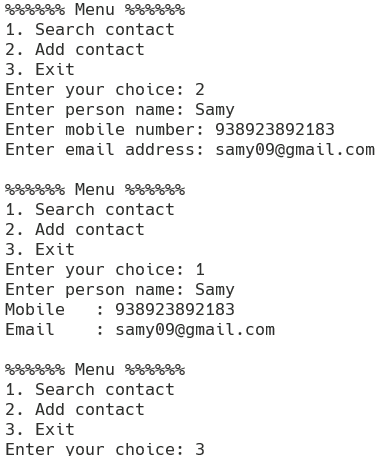
\includegraphics[width=0.6\columnwidth]{P1.png}
  \end{figure}

  \subsection*{Problema 2}
  Construya el algoritmo de la \textit{Constante de Kaprekar} que esta descrito en: \url{https://edabit.com/challenge/eBkknBKXvMm8bDo8M} 

  Realice una conexión Socket en java donde el cliente coloque un numero de cuatro dígitos y el servidor conteste $n$, donde $n$ es el numero de pasos que se usaron para llegar a la \textit{Constante de Kraprekar}.

  Dicha consulta se deberá guardar en un archivo ``Soluciones.txt'', de manera tal que el servidor primero revisará que la solución ya se haya calculada previamente y se haya guardado para ser enviada y si no se calcula al ser una nueva petición.

  \textit{\textbf{Aplicar manejo de archivos, serialización y sockets.}}

  \textit{\textbf{KaprekarServer.java}}
  \begin{lstlisting}
import java.io.*;
import java.net.ServerSocket;
import java.net.Socket;
import java.util.HashMap;
import java.util.Map;
import java.util.Arrays;

public class KaprekarServer {
  private static final String SOLUCIONES_FILE = "Soluciones.txt";
  private static Map<Integer, Integer> solucionesCache = new HashMap<>();

  public static void main(String[] args) {
    try (ServerSocket serverSocket = new ServerSocket(12345)) {
      System.out.println("Servidor esperando conexiones...");

      while (true) {
        Socket clientSocket = serverSocket.accept();
        System.out.println("Cliente conectado: " + clientSocket.getInetAddress());

        try (ObjectInputStream input = 
            new ObjectInputStream(clientSocket.getInputStream());
            ObjectOutputStream output = 
            new ObjectOutputStream(clientSocket.getOutputStream())) {
          int numero = input.readInt();
          int pasos = calcularPasosKaprekar(numero);

          output.writeInt(pasos);
          output.flush();

          guardarEnArchivo(numero, pasos);
        } catch (IOException e) {
          e.printStackTrace();
        }
      }
    } catch (IOException e) {
      e.printStackTrace();
    }
  }

  private static int convertirDigitosEnNumero(int[] digitos) {
    int numero = 0;
    for (int i = 0; i < digitos.length; i++) 
        numero = numero * 10 + digitos[i];
    return numero;
  }

  private static int calcularPasosKaprekar(int numero) {
    int pasos = 0;

    while (numero != 6174) {
      int[] digitos = new int[4];
      for (int i = 3; i >= 0; i--) {
        digitos[i] = numero % 10;
        numero /= 10;
      }

      int[] ascendente = digitos.clone();
      Arrays.sort(ascendente);
      int[] descendente = new int[4];
      for (int i = 0, j = 3; i < 4; i++, j--) 
        descendente[i] = ascendente[j];

      int menor = convertirDigitosEnNumero(ascendente);
      int mayor = convertirDigitosEnNumero(descendente);
      numero = mayor - menor;
      pasos++;
    }

    return pasos;
  }

  private static void guardarEnArchivo(int numero, int pasos) {
    try (BufferedWriter writer = 
        new BufferedWriter(new FileWriter(SOLUCIONES_FILE, true))) {
      writer.write(String.format("%d %d\n", numero, pasos));

      System.out.println("El numero: " + numero + " se tardo " + pasos
          + " pasos en llegar a 6174 y se guardo en el archivo");

      writer.close();
    } catch (IOException e) {
      e.printStackTrace();
    }
  }
}
  \end{lstlisting}

  \textit{\textbf{KaprekarClient.java}}
  \begin{lstlisting}
import java.io.*;
import java.net.Socket;

public class KaprekarClient {
  public static void main(String[] args) {
    try (Socket socket = new Socket("localhost", 12345);
        ObjectOutputStream output = new ObjectOutputStream(socket.getOutputStream());
        ObjectInputStream input = new ObjectInputStream(socket.getInputStream())) {
      int numero;
      do {
        System.out.print("Introduce un numero (0 para salir): ");
        numero = Integer.parseInt(System.console().readLine());
        if (numero == 0) 
          throw new ExitException("Gracias por usar el programa");
        if (numero < 0 || numero > 9999) {
          System.out.println("El numero debe estar entre 0 y 9999");
          continue;
        }
      } while (numero < 0 || numero > 9999);
      output.writeInt(numero);
      output.flush();

      int pasos = input.readInt();
      System.out.println("Numero de pasos para llegar a Kaprekar: " + pasos);
      System.out.println("Gracias por usar el programa");
    } catch (IOException | ExitException e) {
      System.out.println(e.getMessage());
    }
  }
}
  \end{lstlisting}

  \textit{\textbf{ExitException.java}}
  \begin{lstlisting}
public class ExitException extends RuntimeException {
  public ExitException(String message) {
    super(message);
  }
}
  \end{lstlisting}

  \textbf{Ejecución}
  \begin{figure}[h!]
    \centering
    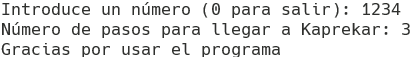
\includegraphics[width=0.8\columnwidth]{P2.png}
  \end{figure}

  \subsection*{Problema 3}
  Cree un archivo de los alumnos de una clase universitaria en dicho archivo deberá contener por línea:
  
  Nombre\$ApellidoPaterno\$ApellidoMaterno $|$ Edad $|$ Estatura $|$ Peso $|$ Promedio $|$ Semestre

  Considere que la edad va de entre 17 a 25 años, la estatura entre 1.45 a 2.00 m., el peso entre 30 a 120 kg, promedio entre 5.0 a 10.0 y el semestre entre 1 a 10.

  Llene el archivo de manera aleatoria, creando 60 casos. Use nombres y apellidos comunes también para llenar cada uno de los registros (al menos 10 apellidos y 10 nombres)

  \begin{enumerate}
    \item Lee el archivo y guarde cada registro como un objeto de tipo Alumno. Aplique el uso de \textit{StringTokenizer} para dividir los campos
    \item Serialice los 60 objetos en el archivo lista.cer.
    \item Deserialice los objetos en un segundo paso y calcule los estadísticos de cada variable numérica:
    \begin{enumerate}[label=\alph*.]
      \item Promedio
      \item Moda
      \item Mediana
    \end{enumerate}
  \end{enumerate}

  \textit{\textbf{Use Scanner y StringTokenizer para manejo de archivos.}}

  \textbf{Solución}
  \begin{lstlisting}
import java.io.BufferedWriter;
import java.io.File;
import java.io.FileInputStream;
import java.io.FileOutputStream;
import java.io.FileWriter;

import java.io.IOException;
import java.io.ObjectInputStream;
import java.io.ObjectOutputStream;
import java.io.Serializable;

import java.util.Random;
import java.util.Scanner;
import java.util.StringTokenizer;
import java.util.ArrayList;

public class Problema3 implements Serializable {
  public static class Alumno implements Serializable {
    String nombre;
    String apellidoPaterno;
    String apellidoMaterno;
    int edad;
    double estatura;
    int peso;
    double promedio;
    int semestre;

    public Alumno(String nombre, String apellidoPaterno, String apellidoMaterno, 
        int edad, double estatura, int peso, double promedio, int semestre) {
      this.nombre = nombre;
      this.apellidoPaterno = apellidoPaterno;
      this.apellidoMaterno = apellidoMaterno;
      this.edad = edad;
      this.estatura = estatura;
      this.peso = peso;
      this.promedio = promedio;
      this.semestre = semestre;
    }
  }

  public static void main(String[] args) {
    String[] nombres = {"Juan", "Maria", "Carlos", "Laura", 
        "Roberto", "Ana", "Pedro", "Sofia", "Miguel", "Elena"};
    String[] apellidos = {"Gomez", "Martinez", "Lopez", "Rodriguez", 
        "Perez", "Garcia", "Fernandez", "Diaz", "Hernandez", "Moreno"};

    final int MINEDAD = 17, MAXEDAD = 25;
    final double MINESTATURA = 1.45, MAXESTATURA = 2.00;
    final int MINPESO = 30, MAXPESO = 120;
    final double MINPROMEDIO = 5.0, MAXPROMEDIO = 10.0;
    final int MINSEMESTRE = 1, MAXSEMESTRE = 10;

    try(BufferedWriter writer = new BufferedWriter(new FileWriter("alumnos.txt"))) {
      Random random = new Random();

      for (int i = 0; i < 60; i++) {
        String nombre = nombres[random.nextInt(nombres.length)];
        String apellidoPaterno = apellidos[random.nextInt(apellidos.length)];
        String apellidoMaterno = apellidos[random.nextInt(apellidos.length)];
        int edad = random.nextInt(MAXEDAD - MINEDAD + 1) + MINEDAD;
        double estatura = MINESTATURA + (MAXESTATURA - MINESTATURA) * random.nextDouble();
        int peso = random.nextInt(MAXPESO - MINPESO + 1) + MINPESO;
        double promedio = MINPROMEDIO + (MAXPROMEDIO - MINPROMEDIO) * random.nextDouble();
        int semestre = random.nextInt(MAXSEMESTRE - MINSEMESTRE + 1) + MINSEMESTRE;

        String linea = String.format("%s | %s| %s | %d | %.2f | %d | %.2f | %d",
            nombre, apellidoPaterno, apellidoMaterno, edad, 
            estatura, peso, promedio, semestre);
        writer.write(linea);
        writer.newLine();
      }

      System.out.println("Archivo creado exitosamente.");

      writer.close();
    } catch(IOException e) {
      e.printStackTrace();
    }

    ArrayList<Alumno> lista = new ArrayList<>();

    try (Scanner scanner = new Scanner(new File("alumnos.txt"))) {
      while (scanner.hasNextLine()) {
        StringTokenizer st = new StringTokenizer(scanner.nextLine(), " | ");
        lista.add(new Alumno(st.nextToken(), st.nextToken(), st.nextToken(),
            Integer.parseInt(st.nextToken()), Double.parseDouble(st.nextToken()),
            Integer.parseInt(st.nextToken()), Double.parseDouble(st.nextToken()),
            Integer.parseInt(st.nextToken())));
      }

      System.out.println("Lista de alumnos creada exitosamente.");
    } catch (IOException e) {
      e.printStackTrace();
    }

    try(ObjectOutputStream oos = 
        new ObjectOutputStream(new FileOutputStream("lista.ser"))) {
      oos.writeObject(lista);
      oos.close();
      System.out.println("Lista de alumnos serializada exitosamente.");
    } catch(IOException e) {
      e.printStackTrace();
    }

    lista.clear();

    try(ObjectInputStream ois = 
        new ObjectInputStream(new FileInputStream("lista.ser"))) {
      lista = (ArrayList) ois.readObject();
      ois.close();
      System.out.println("Lista de alumnos deserializada exitosamente.");
    } catch(IOException | ClassNotFoundException e) {
      e.printStackTrace();
    }  

    double promedio = 
        lista.stream().mapToInt(a -> a.edad).average().getAsDouble();
    System.out.printf("\nPromedio de edad: %.2f\n",  promedio);
    int moda = 
        lista.stream().mapToInt(a -> a.edad).max().getAsInt();
    System.out.println("Moda de edad: " + moda);
    int mediana = 
        lista.stream().mapToInt(a -> a.edad).sorted().toArray()[lista.size() / 2];
    System.out.println("Mediana de edad: " + mediana);

    promedio = 
        lista.stream().mapToDouble(a -> a.estatura).average().getAsDouble();
    System.out.printf("\nPromedio de estatura: %.2f\n", promedio);
    double modaEstatura =   
        lista.stream().mapToDouble(a -> a.estatura).max().getAsDouble();
    System.out.println("Moda de estatura: " + modaEstatura);
    double medianaEstatura = 
        lista.stream().mapToDouble(a -> a.estatura).sorted().toArray()[lista.size() / 2];
    System.out.println("Mediana de estatura: " + medianaEstatura);

    promedio =  
        lista.stream().mapToInt(a -> a.peso).average().getAsDouble();
    System.out.printf("\nPromedio de peso: %.2f\n", promedio);
    moda = 
        lista.stream().mapToInt(a -> a.peso).max().getAsInt();
    System.out.println("Moda de peso: " + moda);
    mediana = 
        lista.stream().mapToInt(a -> a.peso).sorted().toArray()[lista.size() / 2];
    System.out.println("Mediana de peso: " + mediana);

    promedio = 
        lista.stream().mapToDouble(a -> a.promedio).average().getAsDouble();
    System.out.printf("\nPromedio de peso: %.2f\n", promedio);
    double modaPromedio = 
        lista.stream().mapToDouble(a -> a.promedio).max().getAsDouble();
    System.err.println("Moda de promedio: " + modaPromedio);
    double medianaPromedio = 
        lista.stream().mapToDouble(a -> a.promedio).sorted().toArray()[lista.size() / 2];
    System.err.println("Mediana de promedio: " + medianaPromedio);

    promedio = 
        lista.stream().mapToInt(a -> a.semestre).average().getAsDouble();
    System.out.printf("\nPromedio de peso: %.2f\n", promedio);
    moda = 
        lista.stream().mapToInt(a -> a.semestre).max().getAsInt();
    System.err.println("Moda de semestre: " + moda);
    mediana = 
        lista.stream().mapToInt(a -> a.semestre).sorted().toArray()[lista.size() / 2];
    System.err.println("Mediana de semestre: " + mediana);
  }
}
  \end{lstlisting}

  \textbf{Ejecución}
  \begin{figure}[h!]
    \centering
    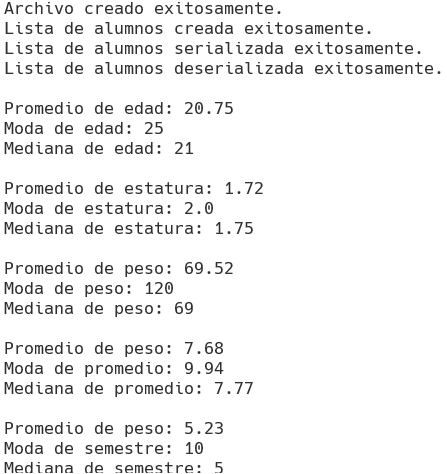
\includegraphics[width=0.75\columnwidth]{P3.png}
  \end{figure}

  \subsection*{Problema 4}
  Realice un verificador de copias de archivos. Este programa leerá dos archivos txt diferentes o iguales y calculará la similitud entre ellos.

  \textit{\textbf{Use manejo de archivos y una expresión lambda de tipo función para realizar dicho algoritmo.}}

  \textbf{Solución}
  \begin{lstlisting}
import java.io.BufferedReader;
import java.io.FileReader;
import java.io.IOException;
import java.util.HashSet;
import java.util.Set;

public class Problema4 {
  public static void main(String[] args) {
    String archivo1 = "./archivo1.txt";
    String archivo2 = "./archivo2.txt";

    try {
      double similitud = calcularSimilitud(archivo1, archivo2);
      System.out.println("La similitud entre los archivos es: " + 
          String.format("%.2f", similitud * 100) + "%");
    } catch (IOException e) {
      e.printStackTrace();
    }
  }

  private static double calcularSimilitud(String archivo1, String archivo2) 
    throws IOException {
    Set<String> conjunto1 = leerArchivo(archivo1);
    Set<String> conjunto2 = leerArchivo(archivo2);

    Set<String> interseccion = new HashSet<>(conjunto1);
    interseccion.retainAll(conjunto2);

    Set<String> union = new HashSet<>(conjunto1);
    union.addAll(conjunto2);

    return (double) interseccion.size() / union.size();
  }

  private static Set<String> leerArchivo(String archivo) 
      throws IOException {
    try (BufferedReader br = new BufferedReader(new FileReader(archivo))) {
      return br.lines().map(String::toLowerCase).
      collect(HashSet::new, Set::add, Set::addAll);
    }
  }
}
  \end{lstlisting}

  \textit{\textbf{archivo1.txt}} 

  \begin{tiny}
    \ttfamily

    Elit in do ut consectetur amet eiusmod officia tempor incididunt. Dolor laborum cupidatat laborum reprehenderit nisi nostrud non veniam ut anim. Esse enim incididunt esse eiusmod veniam enim anim eu nulla pariatur dolor. Dolor nostrud do duis adipisicing dolor aute aliqua consequat cupidatat exercitation. Tempor velit nulla ea nisi fugiat pariatur fugiat eiusmod duis incididunt cillum labore magna reprehenderit. Ea nulla aliqua cupidatat nulla magna qui nisi.
  \end{tiny}

  \textit{\textbf{archivo2.txt}}

  \begin{tiny}
    \ttfamily
    
    Elit in do ut consectetur amet eiusmod officia tempor incididunt. Dolor laborum cupidatat laborum reprehenderit nisi nostrud non veniam ut anim. Esse enim incididunt esse eiusmod veniam enim anim eu nulla pariatur dolor. Dolor nostrud do duis adipisicing dolor aute aliqua consequat cupidatat exercitation. Tempor velit nulla ea nisi fugiat pariatur fugiat eiusmod duis incididunt cillum labore magna reprehenderit. Ea nulla aliqua cupidatat nulla magna qui nisi.
  \end{tiny}

  \begin{tiny}
    \ttfamily

    Dolor laborum cupidatat laborum reprehenderit nisi nostrud non veniam ut anim. Esse enim incididunt esse eiusmod veniam enim anim eu nulla pariatur dolor. Dolor nostrud do duis adipisicing dolor aute aliqua consequat cupidatat exercitation. Tempor velit nulla ea nisi fugiat pariatur fugiat eiusmod duis incididunt cillum labore magna reprehenderit. Ea nulla aliqua cupidatat nulla magna qui nisi.
  \end{tiny}

  \textbf{Ejecución}
  \begin{figure}[h!]
    \centering
    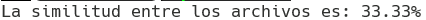
\includegraphics[width=\columnwidth]{P4.png}
  \end{figure}

  \section*{Conclusiones}
  En la experiencia de abordar el manejo de archivos en la programación orientada a objetos, hemos fortalecido nuestra habilidad para crear, leer y escribir datos de manera efectiva. La utilización de clases fundamentales como \textit{File}, \textit{FileOutputStream}, entre otras, junto con la comprensión de flujos de bytes y caracteres, nos ha dotado de herramientas esenciales.

  Las variables de tipo \textit{transient} se emplean para señalar que los características de un objeto no forman parte permanente del mismo, o bien, que no es necesario almacenar y recuperar estos atributos mediante el procedimiento de serialización convencional.

  La variedad de clases, la administración de archivos a través de \textit{File}, y la interacción con flujos de datos han enriquecido nuestra capacidad para gestionar información proveniente de diversas fuentes. La aplicación de técnicas como la serialización ha mejorado la eficiencia al preservar estados de objetos.

  En resumen, este proceso no solo requiere habilidades técnicas, sino también una comprensión profunda de la estructura de datos, lo que optimiza la manipulación de archivos y sienta las bases para aplicaciones más sólidas y eficientes.

  \section*{Referencias}
  \begin{small}
    \textit{Edabit.} (2023). Edabit.com. \url{https://edabit.com/challenge/eBkknBKXvMm8bDo8M} \\

    Solano, J. (2017, 20 enero). \textit{Manual de prácticas de Programación Orientada a Objetos}. Laboratorio de Computación Salas A y B. \url{http://lcp02.fi-b.unam.mx/} \\
  \end{small}
\end{document}